\subsection{Unbearbeitete Spektren}
In den folgenden Darstellungen der Spektren wird auf Fehlerangaben verzichtet.
\begin{figure}[h]
  \centering
  \begin{subfigure}[h]{0.5\textwidth}
    \centering
    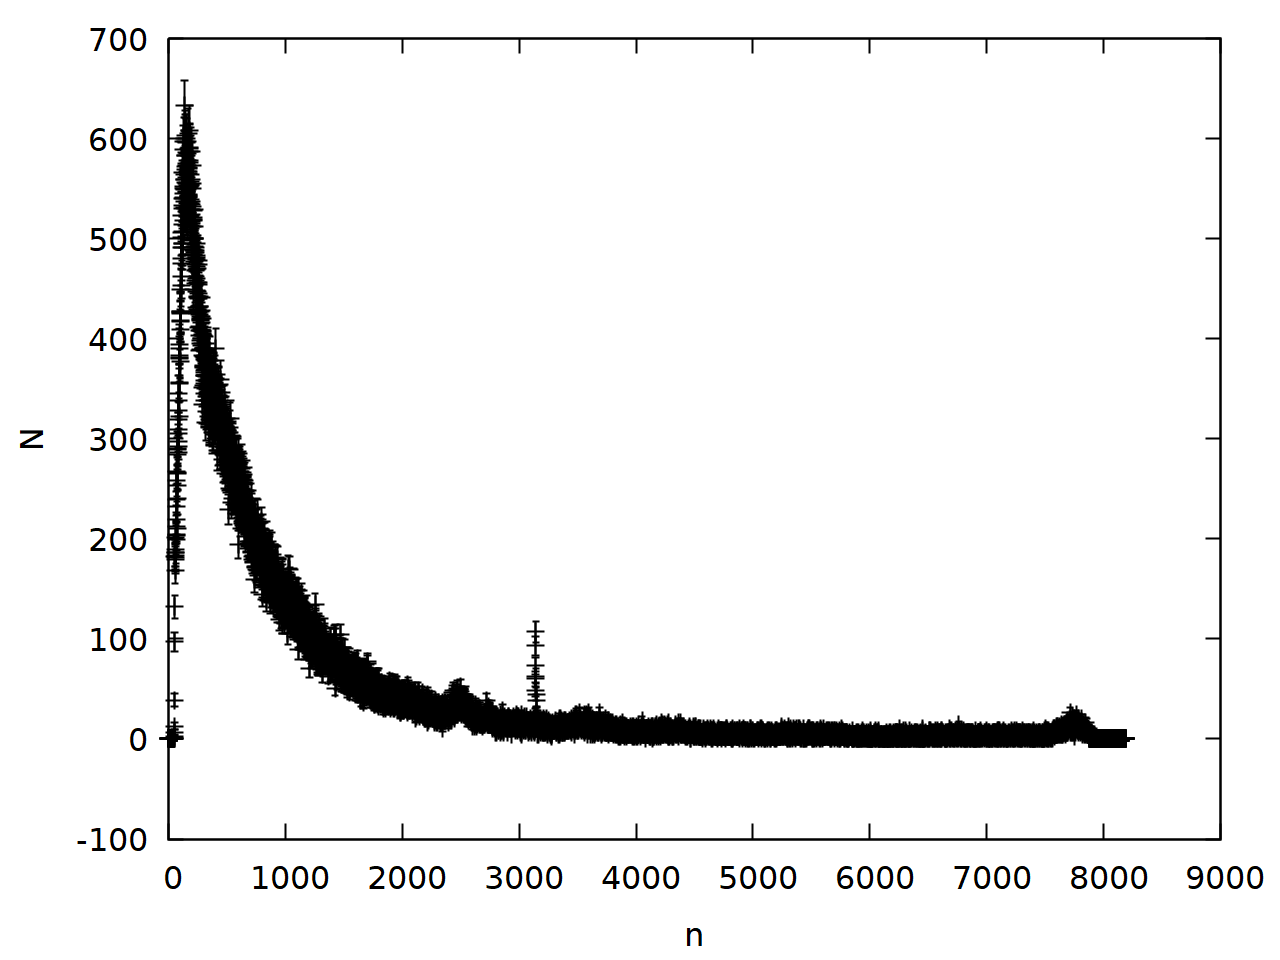
\includegraphics[width=\textwidth]{data/si_unter.png}
    \caption{Szintilationsdetektor}
  \end{subfigure}%
  \begin{subfigure}[h]{0.5\textwidth}
    \centering
    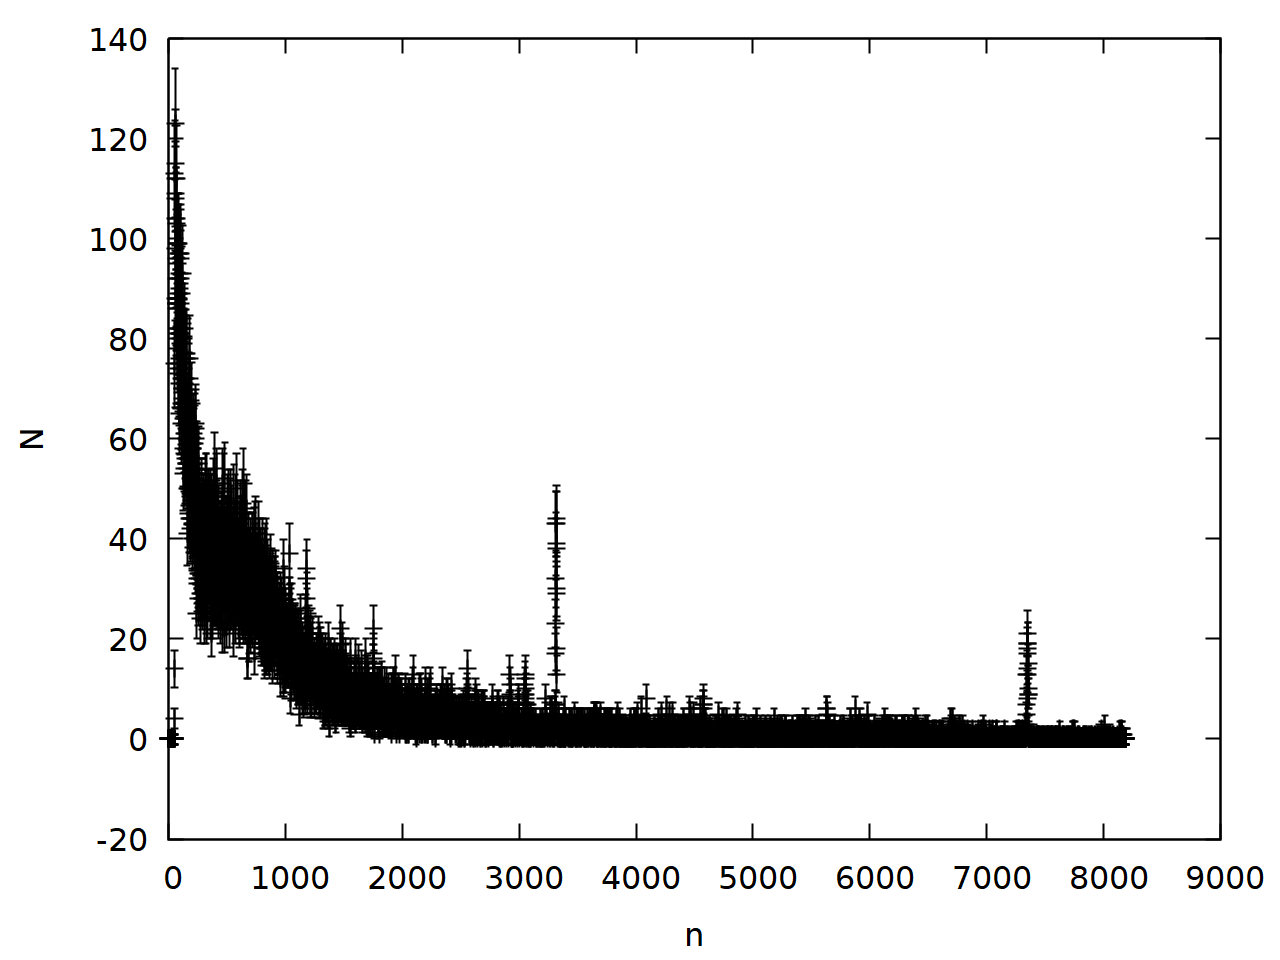
\includegraphics[width=\textwidth]{data/ge_unter.png}
    \caption{Halbleiterdetektor}
  \end{subfigure}
  \caption{Untergrundmessung}
\end{figure}

\begin{figure}[h]
  \centering
  \begin{subfigure}[h]{0.5\textwidth}
    \centering
    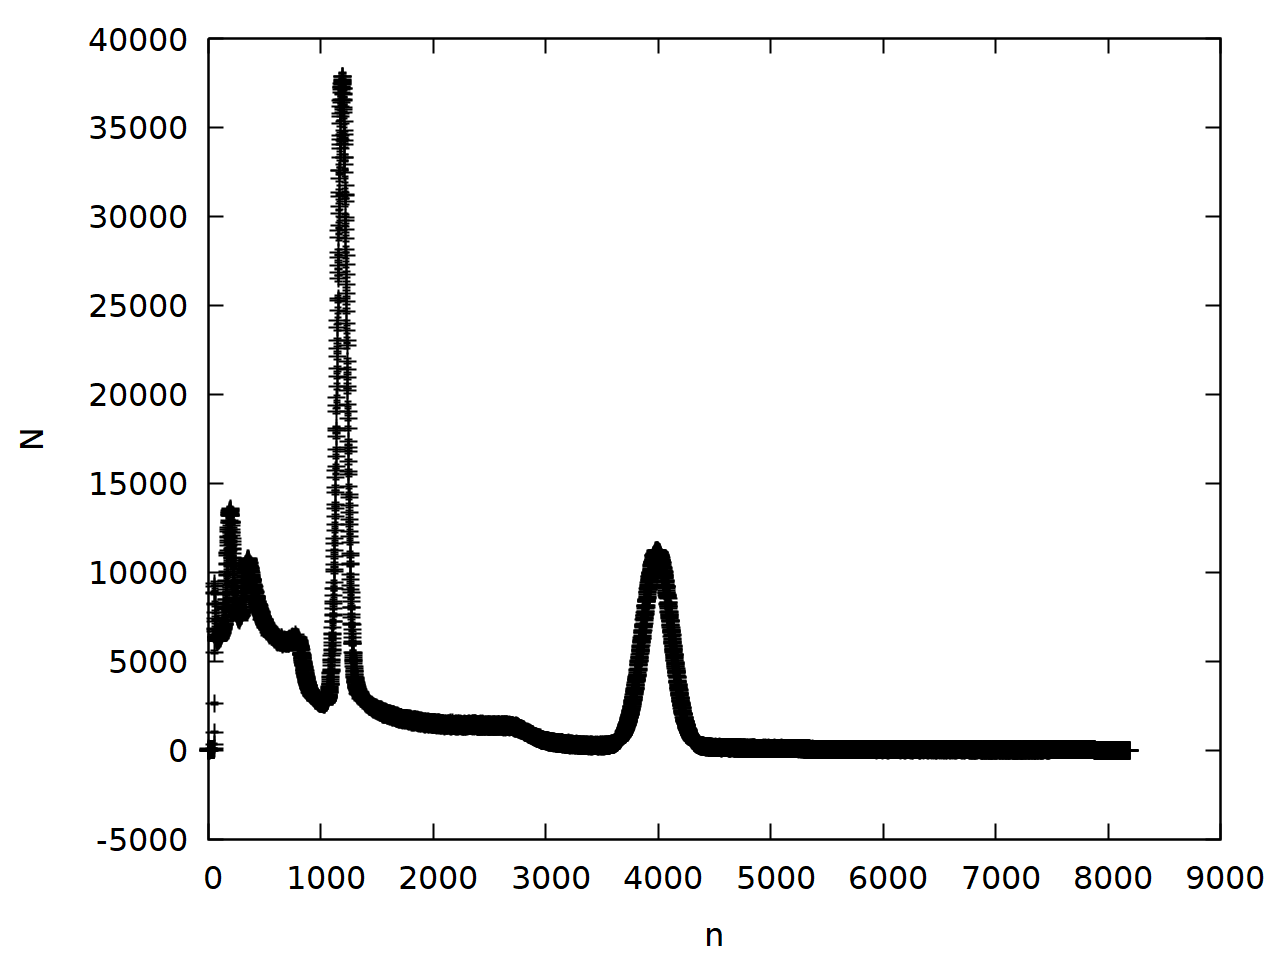
\includegraphics[width=\textwidth]{data/si_cs_raw.png}
    \caption{Szintilationsdetektor}
  \end{subfigure}%
  \begin{subfigure}[h]{0.5\textwidth}
    \centering
    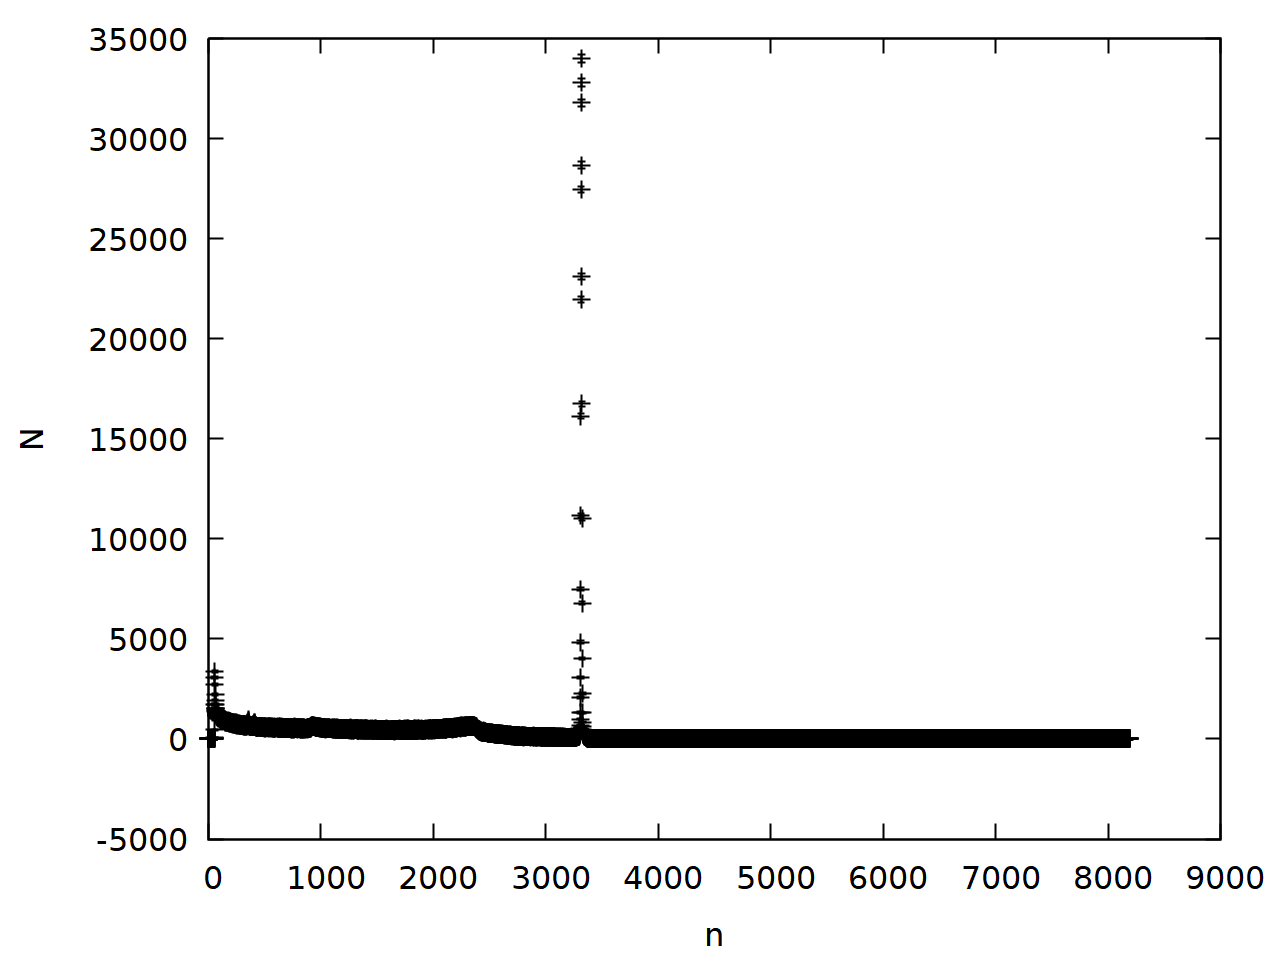
\includegraphics[width=\textwidth]{data/ge_cs_raw.png}
    \caption{Halbleiterdetektor}
  \end{subfigure}
  \caption{Cs-Spektrum}
\end{figure} 

\begin{figure}[h]
  \centering
  \begin{subfigure}[h]{0.5\textwidth}
    \centering
    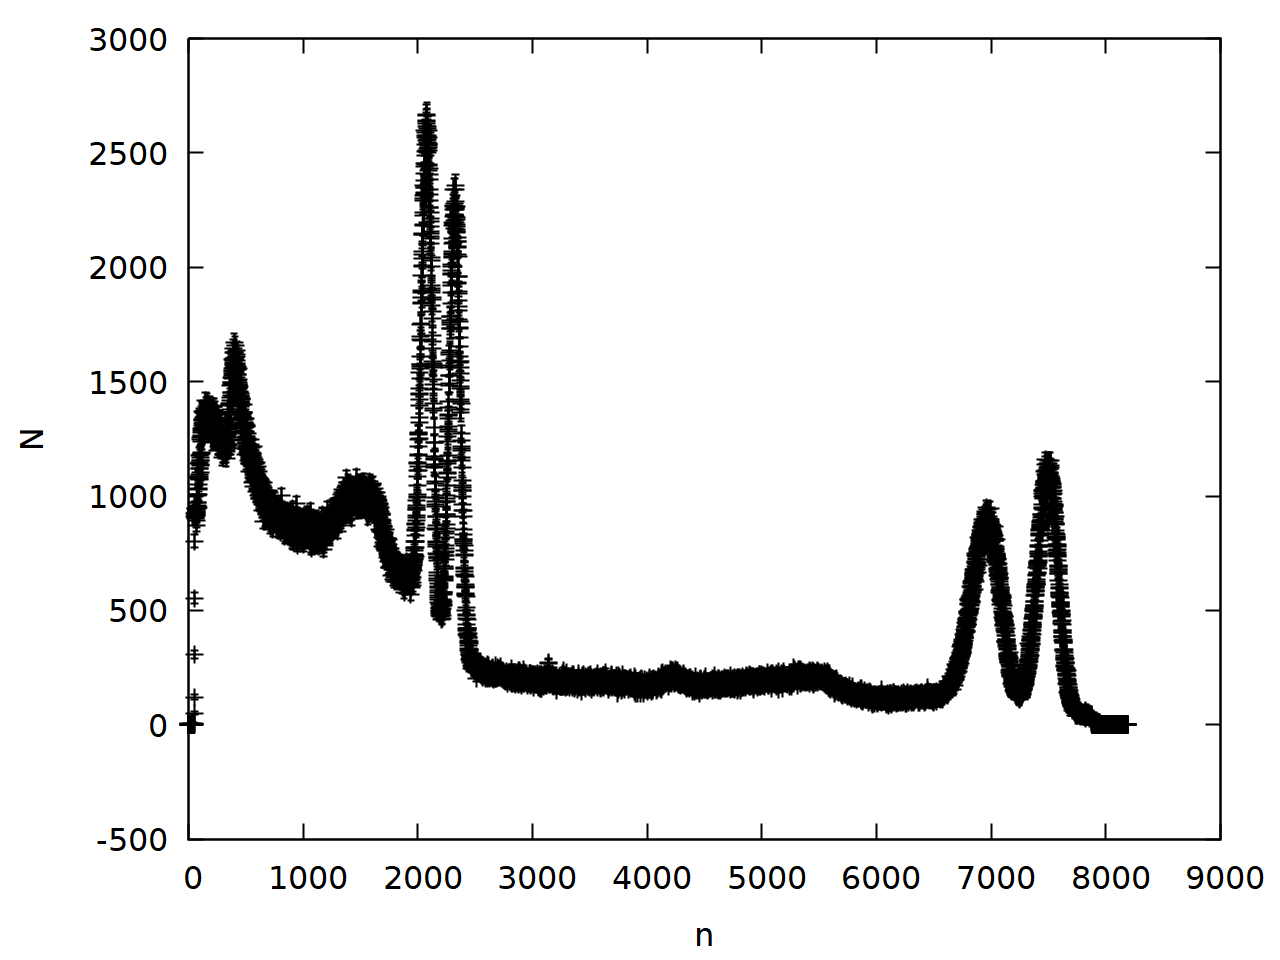
\includegraphics[width=\textwidth]{data/si_co_raw.png}
    \caption{Szintilationsdetektor}
  \end{subfigure}%
  \begin{subfigure}[h]{0.5\textwidth}
    \centering
    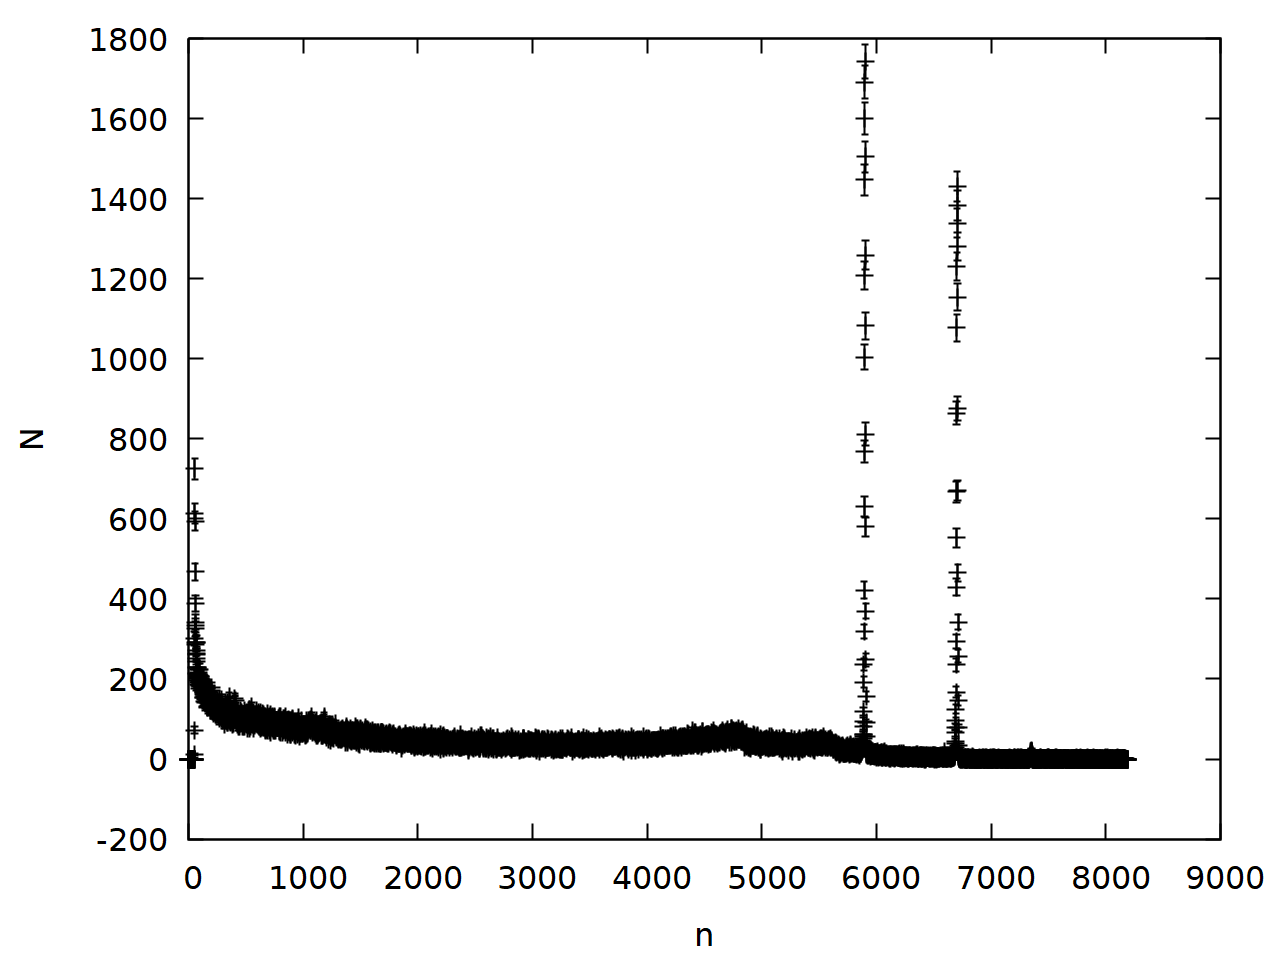
\includegraphics[width=\textwidth]{data/ge_co_raw.png}
    \caption{Halbleiterdetektor}
  \end{subfigure}
  \caption{Co-Spektrum}
\end{figure}

\begin{figure}[h]
  \centering
  \begin{subfigure}[h]{0.5\textwidth}
    \centering
    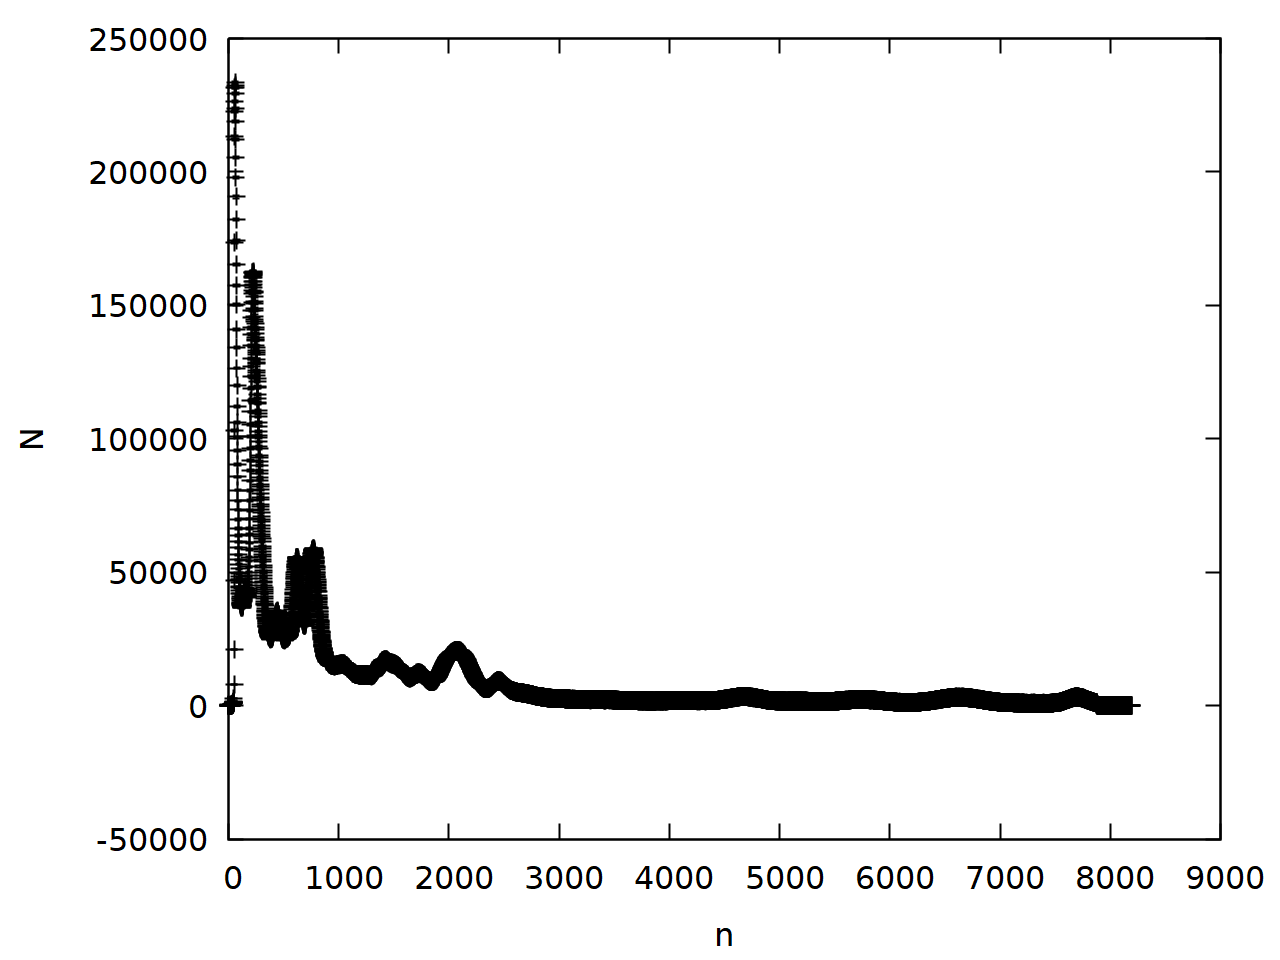
\includegraphics[width=\textwidth]{data/si_eu_raw.png}
    \caption{Szintilationsdetektor}
  \end{subfigure}%
  \begin{subfigure}[h]{0.5\textwidth}
    \centering
    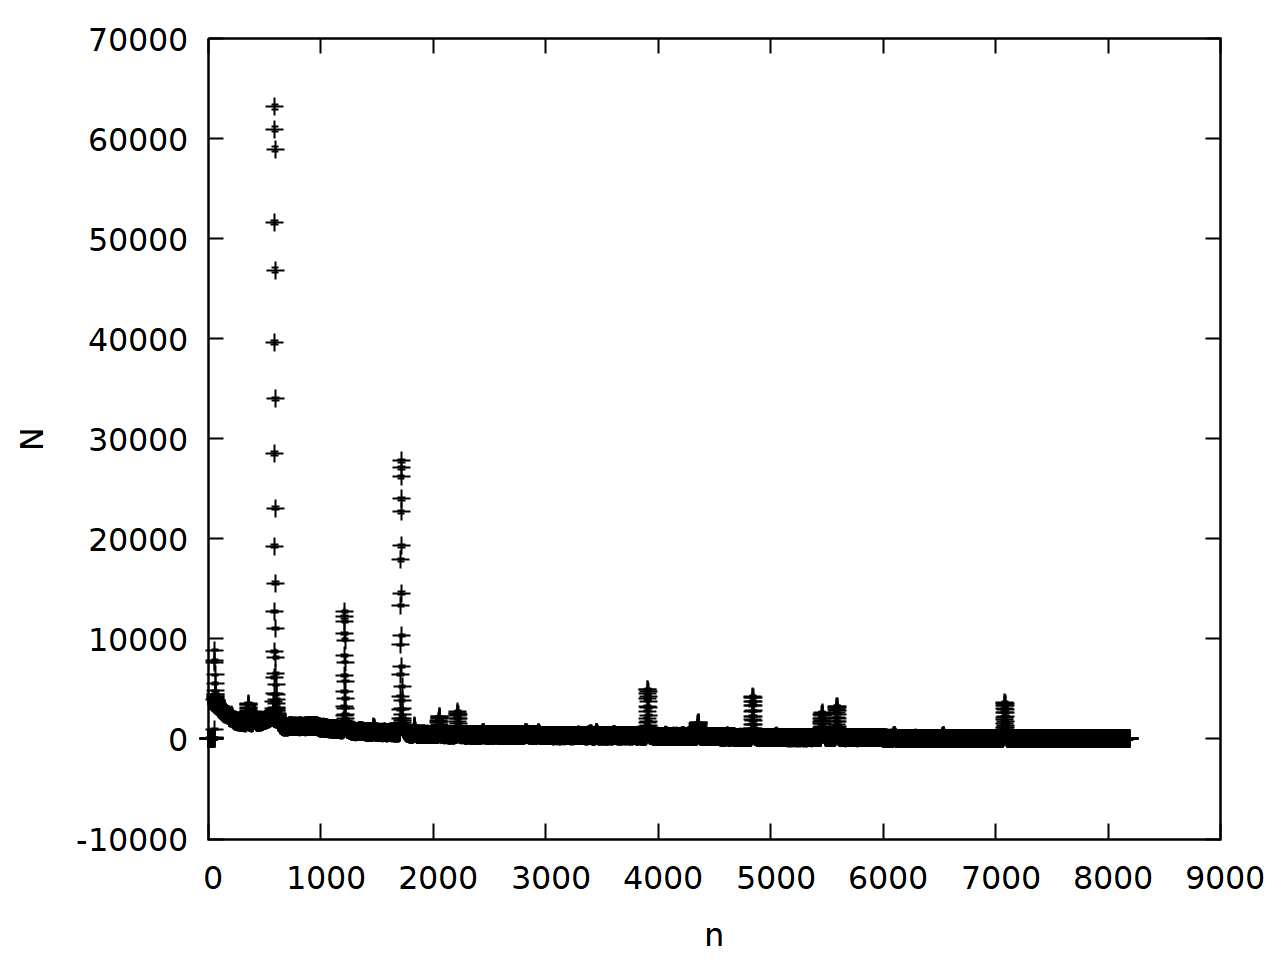
\includegraphics[width=\textwidth]{data/ge_eu_raw.png}
    \caption{Halbleiterdetektor}
  \end{subfigure}
  \caption{Eu-Spektrum}
\end{figure}

\begin{figure}[h]
  \centering
  \begin{subfigure}[h]{0.5\textwidth}
    \centering
    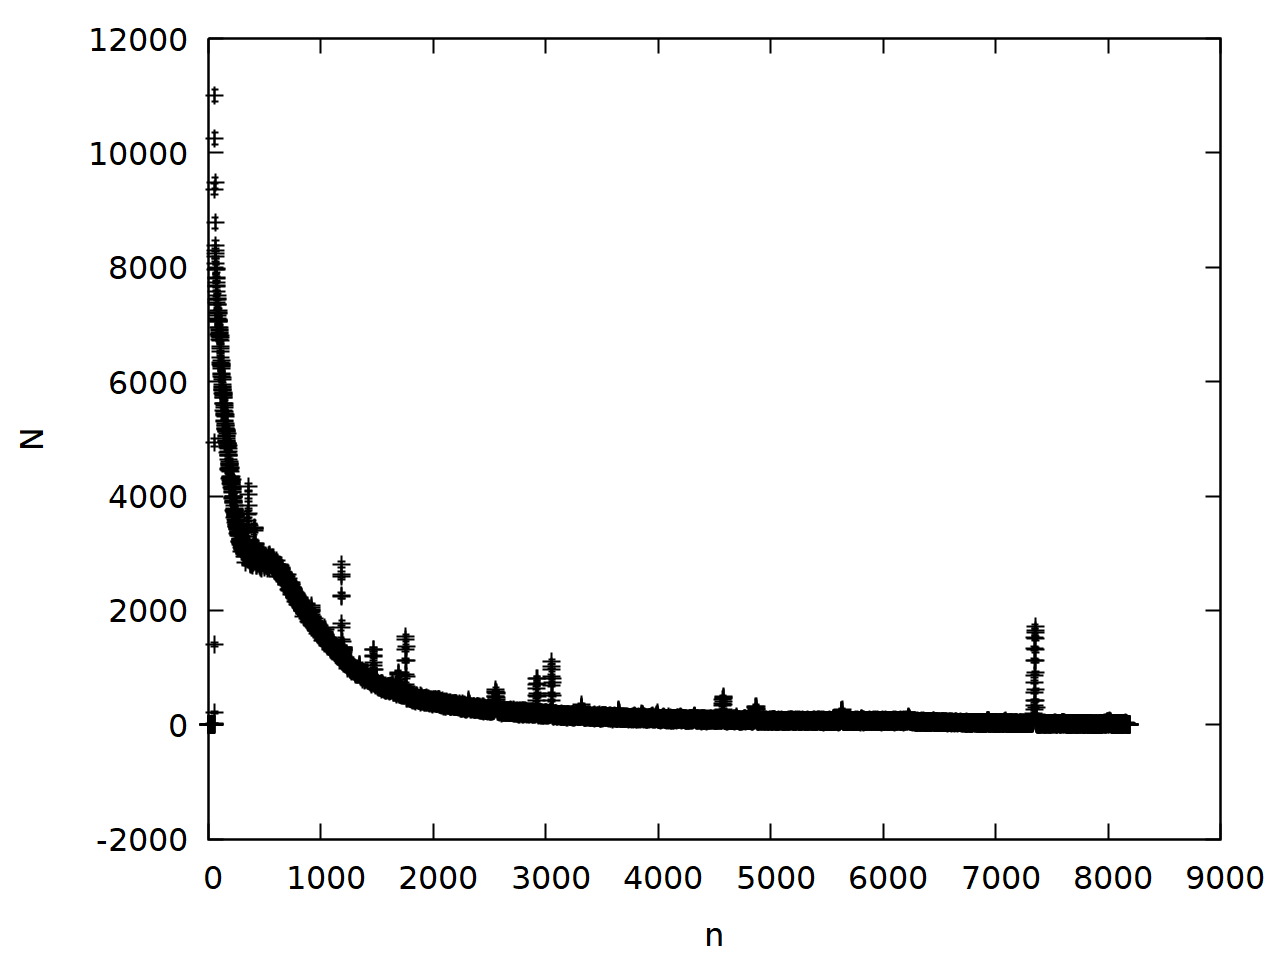
\includegraphics[width=\textwidth]{data/untergrund.png}
    \caption{Untergrund}
  \end{subfigure}%
  \begin{subfigure}[h]{0.5\textwidth}
    \centering
    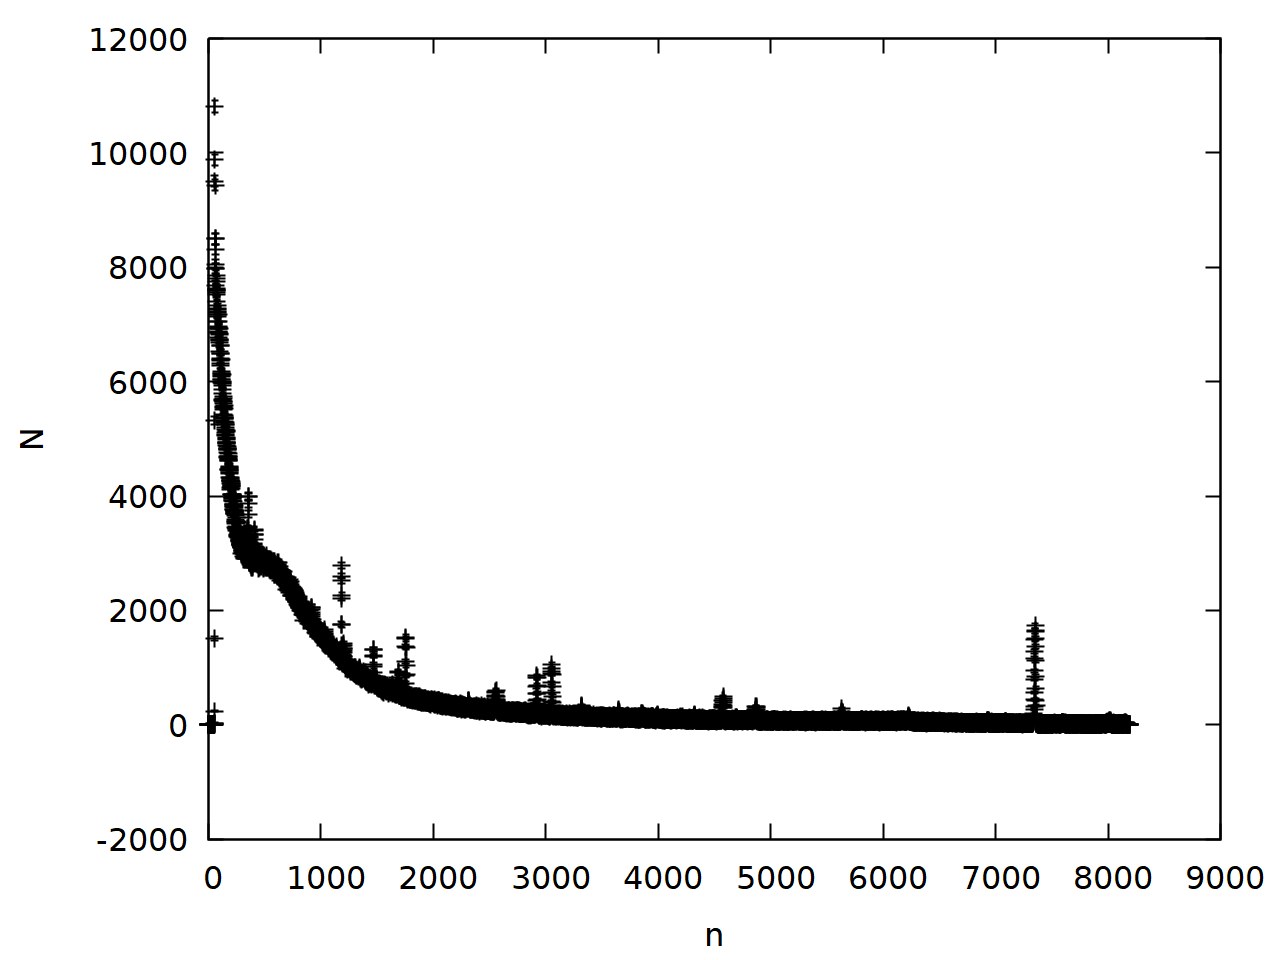
\includegraphics[width=\textwidth]{data/erde_raw.png}
    \caption{Bodenprobe}
  \end{subfigure}
  \caption{Spektren aus Langzeitmessung mit Halbleiterdetektor}
\end{figure}
